%%%%%%%%%%%%%%%%%%%%%%%%%%%%%%%%%%%%%%%%%%%%%%%%%%%%%
% 75.45 Taller de Desarrollo de Proyectos I
% Weepo - Carpet de proyecto
% Facultad de Ingeniería
% Universidad de Buenos Aires
%
% Version 0.1 (07/08/2015)
%
% Original authors:
% 
% Fabrizio Graffe (COMPLETAR@gmail.com)
% Daniel Fernández (COMPLETAR@gmail.com)
% Agustin Rojas (rojasagustin90@gmail.com)
% Jasmina Sella Faena (jasminasf@gmail.com)
% Ezequiel Reyes (COMPLETAR@gmail.com)
% Federico Martin Rossi (federicomrossi@gmail.com)
%
%%%%%%%%%%%%%%%%%%%%%%%%%%%%%%%%%%%%%%%%%%%%%%%%%%%%%



%------------------------------------------------------------------------------
%	PACKAGES AND OTHER DOCUMENT CONFIGURATIONS
%------------------------------------------------------------------------------

\documentclass[oneside]{book}

% Paquetes generales
\usepackage[left=4cm, right=3cm, top=4cm, bottom=3cm, paperwidth=210mm, paperheight=297mm, headsep=1.5cm]{geometry}
\usepackage[utf8]{inputenc}
\usepackage[svgnames]{xcolor} % Required to specify font color
\usepackage{gensymb}

% Paquetes para estilos
\usepackage{textcomp}
\usepackage{setspace}
\usepackage{colortbl}
\usepackage{color}
\usepackage{color}
\usepackage{upquote}
\usepackage{xcolor}
\usepackage{listings}
\usepackage{caption}
\usepackage[T1]{fontenc}
\usepackage[scaled]{beramono}
\usepackage{listings}

% Paquetes extras
\usepackage{amssymb}
\usepackage{float}
\usepackage{graphicx}
\usepackage[export]{adjustbox}
\usepackage{url}
\usepackage[toc,page]{appendix}

% Paquete Matematica
\usepackage{mathtools}

% Paquetes para header y footer
\usepackage{fancyhdr}



% Definición de preferencias para la impresión de código fuente.
%% Colores
\definecolor{gray99}{gray}{.99}
\definecolor{gray95}{gray}{.95}
\definecolor{gray85}{gray}{.85}
\definecolor{gray75}{gray}{.75}
\definecolor{gray50}{gray}{.50}
\definecolor{keywords_blue}{rgb}{0.13,0.13,1}
\definecolor{comments_green}{rgb}{0,0.5,0}
\definecolor{strings_red}{rgb}{0.9,0,0}




% \usepackage{titlesec}

% \titleformat*{\section}{\LARGE\bfseries}
% \titleformat*{\subsection}{\Large\bfseries}
% \titleformat*{\subsubsection}{\large\bfseries}
% \titleformat*{\paragraph}{\large\bfseries}
% \titleformat*{\subparagraph}{\large\bfseries}

% Ocultamos numeración de las secciones
% \setcounter{secnumdepth}{0}



\renewcommand{\chaptername}{Capítulo}
\renewcommand{\contentsname}{Contenido}
% \titleformat{\chapter}[display]
%   {\normalfont\bfseries\huge\color{black}}
%   {\chaptertitlename\ \thechapter}{0.5em}{\textbf\Huge} 
% \titleformat{\section}
%   {\normalfont\Large\fontfamily{fvs}\bfseries\color{black}}
%   {\thesection}{1em}{\Large}
% \titleformat{\subsection}
%   {\normalfont\Large\fontfamily{fvs}\color{cyan}}
%   {\thesection}{1em}{\Large}

% \titleformat{\chapter}[hang] 
% {\normalfont\Huge\fontfamily{fvs}}{\chaptertitlename\ \thechapter:}{0.5em}{\Huge} 
% \titleformat{\section}{\normalfont\Large\fontfamily{fvs}}{\thesection}{1em}{\Large}



%% Caja de código
\DeclareCaptionFont{white}{\color{white}}
\DeclareCaptionFont{style_labelfont}{\color{black}\textbf}
\DeclareCaptionFont{style_textfont}{\it\color{black}}
\DeclareCaptionFormat{listing}{\colorbox{gray95}{\parbox{13.80cm}{#1#2#3}}}
\captionsetup[lstlisting]{format=listing,labelfont=style_labelfont,textfont=style_textfont}

\lstset{
	aboveskip = {1.5\baselineskip},
	backgroundcolor = \color{gray99},
	basicstyle = \ttfamily\footnotesize,
	breakatwhitespace = true,   
	breaklines = true,
	captionpos = t,
	columns = fixed,
	commentstyle = \color{comments_green},
	escapeinside = {\%*}{*)}, 
	extendedchars = true,
	frame = lines,
	keywordstyle = \color{keywords_blue}\bfseries,
	language = Java,                       
	numbers = left,
	numbersep = 5pt,
	numberstyle = \tiny\ttfamily\color{gray50},
	prebreak = \raisebox{0ex}[0ex][0ex]{\ensuremath{\hookleftarrow}},
	rulecolor = \color{gray75},
	showspaces = false,
	showstringspaces = false, 
	showtabs = false,
	stepnumber = 1,
	stringstyle = \color{strings_red},                                    
	tabsize = 2,
	title = \null, % Default value: title=\lstname
	upquote = true,                  
}

%% FIGURAS
\captionsetup[figure]{labelfont=bf,textfont=it}
%% TABLAS
\captionsetup[table]{labelfont=bf,textfont=it}

% COMANDOS

%% Titulo de las cajas de código
\renewcommand{\lstlistingname}{Código}
%% Titulo de las figuras
\renewcommand{\figurename}{Imagen}
%% Titulo de las tablas
\renewcommand{\tablename}{Tabla}
%% Referencia a los códigos
\newcommand{\refcode}[1]{\textit{Código \ref{#1}}}
%% Referencia a las imagenes
\newcommand{\refimage}[1]{\textit{Imagen \ref{#1}}}




%------------------------------------------------------------------------------
%	HEADER AND FOOTER
%------------------------------------------------------------------------------


% \pagestyle{fancy}

% \lhead{}
% \chead{}
% \rhead{}
% \lfoot{}
% \cfoot{}
% \rfoot{}



%------------------------------------------------------------------------------
%	BLANK DOCUMENT
%------------------------------------------------------------------------------

\begin{document}

\pagenumbering{roman}
% \setcounter{page}{0}

% \pagestyle{empty} % Removes page numbers
\thispagestyle{empty}



% TÍTULO, AUTORES Y FECHA
\begin{titlepage}
	\vspace*{\fill}
	\begin{center}
		\Huge{Weepo} \\
		\medskip
		\huge \textit{``Carpeta de proyecto''} \\
		
		\bigskip\bigskip\bigskip\bigskip\bigskip\bigskip

		\Large Fabrizio Graffe, Padrón Nro. 93.158 \\
		\large \textit{zebas,graffe@gmail.com} \\ \medskip
		
		\Large Daniel Fernández, Padrón Nro. 93.083 \\
		\large \textit{COMPLETAR@gmail.com} \\ \medskip
		
		\Large Agustin Rojas, Padrón Nro. 90.000 \\
		\large \textit{rojasagustin90@gmail.com} \\ \medskip

		\Large Jasmina Sella Faena, Padrón Nro. 91.958 \\
		\large \textit{jasminasf@gmail.com} \\ \medskip

		\Large Ezequiel Reyes, Padrón Nro. 90.000 \\
		\large \textit{COMPLETAR@gmail.com} \\ \medskip
		
		\Large Federico Martín Rossi, Padrón Nro. 92.086 \\
		\large \textit{federicomrossi@gmail.com} \\

		\bigskip\bigskip\bigskip\bigskip\bigskip\bigskip

		\large 1er. Cuatrimestre 2015 \\ \smallskip
		\large 75.45 Taller de Desarrollo de Proyectos I \\ \smallskip
		\large Facultad de Ingeniería, Universidad de Buenos Aires \\ \smallskip

		\date{}
	\end{center}
	\vspace*{\fill}
\end{titlepage}




%
% TEXTOS PREVIOS
%
\section*{\bfseries\color{black}Antes de empezar}

Los diagramas en los cuales se basarán y apoyarán las explicaciones de este informe se encuentran modelados con \textit{UML} mientras que los fragmentos de código que muestran la implementación de los distintos modelos se realizarán en el lenguaje de programación \textit{Java}. Por esta razón, este informe asume que el lector posee conocimientos básicos de \textit{Programación Orientada a Objetos}, \textit{Java} y \textit{UML}.
\bigskip


\section*{\bfseries\color{black}Repositorio del grupo}

Todos los archivos y códigos fuente aquí mencionados, así como también el presente informe, pueden ser descargados del repositorio del grupo ubicado en  \url{https://bitbucket.org/7510201402g14}.
\bigskip



% ÍNDICE
\tableofcontents
%\clearpage\null\newpage

\pagenumbering{arabic}
\setcounter{page}{0}
\thispagestyle{empty}





\chapter{An\'{a}lsis comercial}


\section{Intro}

Con el auge de las redes sociales se han abierto nuevas oportunidades de negocios. Esto ha fomentado el interés de poder promocionar campañas de marketing desde distintos sectores.
El problema surge cuando se necesita seleccionar a los individuos ideales para realizar una correcta promoci\'{o}n.


\section{Alcance}

\begin{itemize}

\item Marcas con intenci\'{o}n de publicitar tendr\'{a}n uno perfil en el cual podr\'{a}n administrar sus campañas publicitarias en distintas redes sociales.

\item Cada marca podr\'{a} registrar a una lista de usuarios, que ser\'{a}n los encargados de administrar el perfil de la marca. Cada usuario podr\'{a} ver informaci\'{o}n general de la marca e informaci\'{o}n propia, pero no de otros usuarios de dicha marca ni de ninguna otra. 

\item Cada campa\~{n}a constar\'{a} de ciertos factores definidos por el usuario, los cuales apuntan a definir la estrategia de generaci\'{o}n de estad\'{i}sticas. De esta forma, el usuario especificar\'{a} hacia donde desea apuntar su plan de negocio y/o marketing.

\item Las caracter\'{i}sticas que se podrán especificar son: red social, rangos de edad, ubicación (pa\'{i}s, ciudad, estado / provincia), Género (femenino, masculino, gays, etc.), entretenimiento (g\'{e}nero de música, serie de televisi\'{o}n, libros, etc.).

\item Una vez especificadas las caracter\'{i}sticas, se generar\'{a} una estad\'{i}stica por cada red social agregada en la cual emerger\'{a}n los usuarios con m\'{a}s impacto sobre cada red sobre los que conviene apuntar y concentrar la campa\~{n}a. Estos usuarios deber\'{i}an ser quienes provoquen una mayor profundidad y alcance del plan de marketing. 

\item Adem\'{a}s, se generará una estad\'{i}stica central a partir de las estad\'{i}sticas parciales realizadas en cada una de las redes sociales, otorgando una visi\'{o}n global entre estas.

\item Se podr\'{a} obtener a partir de la informaci\'{o}n que se tiene de las redes sociales de las empresas usuario, un listado ordenado de las principales caracter\'{i}sticas o gustos que comparten los seguidores de la marca de dicha empresa.

\item Obtener la opinión o percepción de la marca de la empresa usuario del mercado, realizando an\'{a}lisis de sentimientos en las distintas redes sociales.

\item Generar gráficos y estad\'{i}sticas, tanto actuales como de evoluci\'{o}n en el tiempo acerca de la opini\'{o}n de la marca, teniendo en cuenta la cantidad de opiniones positivas y negativas.

\item Llevar un control de las publicaciones que han sido compartidas.
Seguimiento de hashtags creados (an\'{a}lisis de impacto y de posicionamiento en ranking de trending topic)

\item Permitir publicar y compartir contenido en las diferentes redes sociales, tanto de manera individual como en conjunto. 

\item Análisis de trending topics para la utilización de los hashtags mejor posicionados para impactar sobre los usuarios.
Seguir la actividad de los usuarios de más impacto que son seguidores de la marca. 

\item Ofrecer a las empresas usuario la posibilidad de brindarles los servicios de un asesor de marketing asociado a nuestra web. Para ser parte de nuestros asesores, un aplicante deber\'{a} pasar por una serie de pruebas/entrevistas de manera de garantizar la excelencia de los servicios brindados. 

\item Presentar un conjunto de preguntas frecuentes con sus respuestas, consejos y tips acerca de marketing en redes sociales y cómo mejorar el impacto de la marca en estas.


\end{itemize}


\section{P\'{u}blico}


El sistema esta orientado a:

\begin{enumerate}
	\item Marcas con deseos de publicitar, como pueden ser:
	\begin{itemize}
		\item Cuentapropistas
		\item Emprendimientos 
		\item Pymes
		\item Empresas grandes
	\end{itemize}
	\item Publicistas
	\item Agencias de marketing
	\item Personas del \'{a}mbito pol\'{i}tico que deseen utilizar las redes sociales para incrementar su popularidad. 
\end{enumerate}
 


\section{Ganancias}

Las ganancias ser\'{a}n obtenidas de:
\begin{itemize}
\item La venta del producto con todas sus funcionalidades a las empresas interesadas
\item La venta del producto con algunas de las funcionalidades a los peque\~{n}os emprendedores
\item Existir\'{a} una versión gratuita que incluir\'{a} publicidad y funcionalidades más reducidas
\end{itemize}


\newpage

\section{Análisis de las 5C’s}


\subsection{Compa\~{n}\'{i}a}

	\textbf{Visi\'{o}n:} Ser la empresa de marketing en redes sociales m\'{a}s reconocida y valorada en el mundo. Permitiendo a cada usuario, empresa o emprendimiento, obtener datos y estadísticas sobre su p\'{u}blico objetivo y recomendaciones para sus campa\~{n}as de marketing en redes sociales.\\

	\textbf{Posición:} La empresa es un startup recién establecido. Tiene pocos recursos pero es \'{a}gil.\\

	\textbf{Performance}: La empresa no inici\'{o} actividad a\'{u}n. \\

	\textbf{Línea de productos:}

	\begin{itemize}
		\item An\'{a}lisis del mercado de las marcas. Se estudia el sexo, rangos de edad, información geográfica, etc. de las personas que siguen a la marca de la empresa que utiliza la herramienta. 
		
		\item Análisis de los usuarios con m\'{a}s poder de difusi\'{o}n en una determinada red social, en orden de recomendarlos como usuarios de inter\'{e}s para la empresa que utiliza la herramienta. Generar un ranking con estos.
		
		\item An\'{a}lisis de sentimientos de los mensajes de una red social que mencionan la marca de la empresa que utiliza nuestra herramienta, para as\'{i}, conocer la opini\'{o}n del p\'{u}blico. A su vez se dar\'{a} la posibilidad de leer los mensajes más destacados, un resumen de las opiniones positivas y negativas, etc.
	\end{itemize}


	\textbf{Misión:} Ofrecer una serie de herramientas que permitan a empresas y emprendimientos lanzar una campa\~{n}a de marketing efectiva en las redes sociales, y poder obtener datos y estad\'{i}sticas \'{u}tiles a partir de estas para dicha campa\~{n}a.\\

	\textbf{Objetivos:}

	\begin{itemize}
		\item Proveer un sitio virtual que posea que brinde las herramientas necesarias lograr una campaña de marketing efectiva en las redes sociales para una empresa o emprendimiento.
		
		\item Lograr un posicionamiento l\'{i}der en Argentina como empresa de marketing en redes sociales en un plazo de 6 a\~{n}os.
		
		\item Lograr un posicionamiento l\'{i}der en Latinoam\'{e}rica como empresa de marketing en redes sociales en un plazo de 12 a\~{n}os.
	\end{itemize}

	La estrategia de la organizaci\'{o}n es realizar un proceso iterativo de mejoramiento e incremento de componentes en la aplicaci\'{o}n que permita ser lanzada al mercado al poco tiempo de empezar su implementaci\'{o}n permitiendo así un feedback temprano que se traducir\'{i}a en modificaciones en las fases iniciales del proyecto lo que lograr\'{i}a abaratar costos ya que las modificaciones se realizar\'{a}n en las primeras etapas del proyecto, al mismo tiempo, lanzar la aplicaci\'{o}n al mercado permitir\'{a} obtener un pequeño ingreso de capital lo que será reinvertido en el proyecto adem\'{a}s de generar publicidad con un costo de esta muy reducida.



\subsection{Competidores}
Existen sitios que brindan la posibilidad de manejar perfiles de forma sencilla en distintas redes sociales, así como también existen otras que brindan servicios de análisis de sentimientos en las mismas.\\ 
Se ha hallado una empresa\footnote{\url{https://www.socialmetrix.com}} que brinda los mismos servicios que los que pretende proveer nuestra empresa. Esto puede proveer de una visi\'{o}n del precio de mercado de los servicios. Los costos de los servicios prestados por esta empresa ser\'{a}n mucho mas elevados a los que ofrecer\'{a} nuestra empresa.


\subsection{Clientes}
Los clientes que usen la herramienta brindada serán los siguientes:

\begin{enumerate}
	\item Marcas con deseos de publicitar, como pueden ser:
	\begin{itemize}
		\item Cuentapropistas
		\item Emprendimientos 
		\item Pymes
		\item Empresas grandes
	\end{itemize}
	\item Publicistas
	\item Agencias de marketing
	\item Personas del \'{a}mbito pol\'{i}tico que deseen utilizar las redes sociales para incrementar su popularidad. 
\end{enumerate}


\subsection{Colaboradores}
Se consideran colaboradores de la empresa a los siguientes:
\begin{itemize}
	\item Redes sociales, ya que son las que proveen tanto los datos a ser explotados como los medios para explotarlos (facebook, twitter, linkedin, etc y sus API's).\\
	
	\item Empresas cliente que nos brinden informaci\'{o}n del mercado en el que se manejan, para lograr extraer datos y estadísticas relevantes. \\
	\item APIs de servicios web de bajo costo o gratuitas que brinden funcionalidades de social media analysis.
\end{itemize}




\subsection{Contexto}
No existen restricciones legales que afecten al desarrollo de nuestro servicio ya que no se analiza información que no sea pública o sea de propiedad de las empresas clientes.\\
Las redes sociales cada vez tienen más usuarios y forman una parte importante de la vida de las personas (para bien o para mal), y la información que se puede extraer de estas es muy rica. El  marketing en redes sociales es un área nueva y en pleno desarrollo. Es un momento propicio para el crecimiento de esta industria.




\newpage



\section{An\'{a}lisis de las 4P's}

\subsection{Producto}
El producto consiste en una plataforma de an\'{a}lisis de informaci\'{o}n en redes sociales y sugerencias para lograr una campa\~{n}a de marketing m\'{a}s efectiva en dichas redes.
En particular:

\begin{itemize}
\item Marcas con intenci\'{o}n de publicitar tendr\'{a}n un perfil en el cual podr\'{a}n administrar sus campañas publicitarias en distintas redes sociales.

\item Cada marca podr\'{a} registrar a una lista de usuarios, que ser\'{a}n los encargados de administrar el perfil de la marca. Cada usuario podr\'{a} ver informaci\'{o}n general de la marca e informaci\'{o}n propia, pero no de otros usuarios de dicha marca ni de ninguna otra. 

\item Cada campa\~{n}a constar\'{a} de ciertos factores definidos por el usuario, los cuales apuntan a definir la estrategia de generaci\'{o}n de estad\'{i}sticas. De esta forma, el usuario especificar\'{a} hacia donde desea apuntar su plan de negocio y/o marketing.

\item Las caracter\'{i}sticas que se podrán especificar son: red social, rangos de edad, ubicación (pa\'{i}s, ciudad, estado / provincia), Género (femenino, masculino, gays, etc.), entretenimiento (g\'{e}nero de música, serie de televisi\'{o}n, libros, etc.).

\item Una vez especificadas las caracter\'{i}sticas, se generar\'{a} una estad\'{i}stica por cada red social agregada en la cual emerger\'{a}n los usuarios con m\'{a}s impacto sobre cada red sobre los que conviene apuntar y concentrar la campa\~{n}a. Estos usuarios deber\'{i}an ser quienes provoquen una mayor profundidad y alcance del plan de marketing. 

\item Adem\'{a}s, se generará una estad\'{i}stica central a partir de las estad\'{i}sticas parciales realizadas en cada una de las redes sociales, otorgando una visi\'{o}n global entre estas.

\item Se podr\'{a} obtener a partir de la informaci\'{o}n que se tiene de las redes sociales de las empresas usuario, un listado ordenado de las principales caracter\'{i}sticas o gustos que comparten los seguidores de la marca de dicha empresa.

\item Obtener la opinión o percepción de la marca de la empresa usuario del mercado, realizando an\'{a}lisis de sentimientos en las distintas redes sociales.

\item Generar gráficos y estad\'{i}sticas, tanto actuales como de evoluci\'{o}n en el tiempo acerca de la opini\'{o}n de la marca, teniendo en cuenta la cantidad de opiniones positivas y negativas.

\item Llevar un control de las publicaciones que han sido compartidas.
Seguimiento de hashtags creados (an\'{a}lisis de impacto y de posicionamiento en ranking de trending topic)

\item Permitir publicar y compartir contenido en las diferentes redes sociales, tanto de manera individual como en conjunto. 

\item Análisis de trending topics para la utilización de los hashtags mejor posicionados para impactar sobre los usuarios.
Seguir la actividad de los usuarios de más impacto que son seguidores de la marca. 

\item Ofrecer a las empresas usuario la posibilidad de brindarles los servicios de un asesor de marketing asociado a nuestra web. Para ser parte de nuestros asesores, un aplicante deber\'{a} pasar por una serie de pruebas/entrevistas de manera de garantizar la excelencia de los servicios brindados. 

\item Presentar un conjunto de preguntas frecuentes con sus respuestas, consejos y tips acerca de marketing en redes sociales y cómo mejorar el impacto de la marca en estas.


\end{itemize}


	
\subsection{Precio}
Empresas que brindan servicios de análisis de sentimientos\footnote{\url{https://semantria.com}} en redes sociales ofrecen planes que van desde los US\$900 hasta US\$3000 mensuales. \\
Empresas que ofrecen servicios de marketing en redes sociales\footnote{\url{https://www.socialmetrix.com}} ofrecen planes que van desde los US\$250 hasta los US\$950 por mes.\\
En orden de ganarle mercado a los competidores, los precios deben de ser menores, pero deben seguir siendo tales que generen un ganancia significativa. 


\begin{itemize}
	\item Precio del Producto con plan Premium: 500\$ al mes.

	\item Producto gratuito con funcionalidades reducidas
	\item Precio de customizar la herramienta a medida: A convenir.
Estimado (si es que no es de una dificultad muy superior): \$3000 x funcionalidad extra por \'{u}nica vez.
\end{itemize}






\subsection{Publicidad}
Se comenzará a comunicar el proyecto 3 meses antes del lanzamiento a través de publicidad  online y en publicaciones impresas asociadas al rubro como revistas o sección de tecnología en diarios, etc.
El costo de las mismas está estimado en lo siguiente con sus respectivas fuentes.\\

\begin{itemize}

	\item Publicidad en redes sociales costo estimado: \$13100\footnote{\url{http://www.tecsid.com/publicidad-en-facebook.php}}.
Con esto se lograr\'{a} aproximadamente 10000 likes sobre el anuncio. Teniendo en cuenta que por cada “me gusta”, este anuncio se difundirá entre cada uno de sus respectivos contactos, se podría alcanzar un estimativo del triple de vistas a la misma.

	\item Publicidad a través de Google Adwords\footnote{\url{https://adwords.google.es/select/AfpoFinder?currency=ARS&country=AR
}}, se estima un mínimo de \$40 por d\'{i}a para obtener alrededor de 1000 visitas diarias que a su vez ir\'{a}n incrementando junto con la popularidad del sitio.

	\item Publicidad a trav\'{e}s de youtube mediante videos que promocionen el producto, con un costo aproximado de US\$10 logrando aproximadamente 500 visitas\footnote{\url{http://www.youtube.com/yt/playbook/es-419/promotion.html y http://visitas-youtube.com/planes-y-precios/}}. Tambi\'{e}n se puede realizar publicidad mediante Adwords, es decir, texto que se muestra mientras se reproduce un video, o mediante anuncios InStream que consisten en videos cortos que se muestran durante cinco segundos antes de la reproducción de un video. Luego de cinco segundos, los espectadores pueden seguir viendo el anuncio u omitirlo. Si deciden ver treinta segundos del anuncio como m\'{i}nimo, se paga un “costo por vista”.


Con estos medios de difusión logramos abarcar una gran cantidad de potenciales usuarios. Con un costo que rondará aproximadamente en unos \$25000 por mes.

\end{itemize}






\subsection{Distribuci\'{o}n}
La plataforma ser\'{a} lanzada inicialmente para todos los usuarios hispanoparlantes de latinoam\'{e}rica.
Luego, el sitio será traducido al ingl\'{e}s y nuevas alianzas se harán para alcanzar los territorios m\'{a}s importantes restantes.


\newpage

%
% CAPITULO X
%
\chapter{Tecnologías y metodologías}


% CAPITULO X
\section{Herramientas colaborativas}

	Con el fin de poder llevar a cabo el desarrollo en grupo mediante el soporte necesrio para elaborar el proyecto en forma conjunta y compartida se han utilizado herramientas colaborativas. Estas permiten el intercambio de información, su gestión y control. De esta manera, se logra utilizar el conocimiento táctico y explicito de todo el equipo, generando la posibilidad de gestionar el conocimiento y la participación de cada integrante.
	\par
	Las herramientas elegidas para la organización, comunicación y desarrollo del proyecto han sido:

	\begin{itemize}
	\renewcommand{\labelitemi}{\scriptsize\tiny$\blacksquare$} 
	\itemsep=7pt \topsep=0pt \partopsep=0pt \parskip=0pt \parsep=0pt

		\item \textit{Google Hangouts}\footnote{Mas info sobre Google Hangouts en \url{http://www.google.com/+/learnmore/hangouts/?hl=es-419}}: es una aplicación de mensajería instantánea que permite mantener conversaciones entre dos o más usuarios, como así también videollamadas con hasta 15 personas en web. 
		\par La gran ventaja de este servicio es que todas las conversaciones realizadas se archivan en la nube, permitiéndonos así tener un registro de las temáticas discutidas, y en caso de ser necesario, poder acudir a ellas para tomar nota de ideas o problemáticas surgidas en medio de las charlas. Otra ventaja por la cual se ha optado por este servicio es la posibilidad de compartir a lo largo de la videoconferencia, archivos (imágenes, PDFs, entre otros) potenciando de esta manera el contenido e intercambio en las reuniones.

		\item \textit{Trello}\footnote{Mas info sobre Trello en \url{http://www.trello.com}}: es un gestor de tareas que permite el trabajo en forma colaborativa mediante tableros (boards) dispuestos en columnas (llamadas listas) que representan los distintos estados que pueden tomar las tareas. Se basa en el método Kanban para gestión de proyectos, con tarjetas que viajan por diferentes listas en función de su estado. Así, se puede tener una lista de cosas por hacer (o pendientes), que se están haciendo (están en proceso) o tareas ya terminadas. 
		\par La gran ventaja de este servicio es la de poder visualizar en qué está trabajando cada integrande del proyecto, quién está realizando cada tarea, en que parte del proceso se encuentra cada integrante y globalmente el proyecto. Además permite realizar comentarios sobre cada tarea, manteniendo organizadas las críticas y/o aportes sobre cada una de ellas, como así también, subir archivos asociados a estas.

		\item \textit{GIT}: es un software de control de versiones desarrollado para lograr la eficiencia y la confiabilidad del mantenimiento de versiones de aplicaciones cuando éstas tienen un gran número de archivos de código fuente. GIT permite que todo el equipo de Weepo trabaje en forma conjunta y paralela sobre los archivos.
		\par Se ha utilizado como plataforma de desarrollo colaborativo basado en GIT al servicio \textit{GitHub}.

	\end{itemize}	
\newpage


% CAPITULO X
\section{Stack de desarrollo}

	Se conoce como stack de desarrollo al conjunto de tecnologías que componen la estructura cliente-servidor en toda su extensión. Esta estructura se encuentra dividida en dos partes bien definidas: el lado \textit{Cliente} (o frontend) y el lado \textit{Servidor} (o backend). En la \textit{Imagen X.1} se muestra un avance de todo el conjunto unido y la interconexión que los relaciona. En esta, el backend se encuentra dividido en el servidor web y el servidor de datos, pero para un mejor entendimiento en la explicación, las consideraremos una única unidad.
	\par
	En los siguientes apartados se tratarán dichas divisiones y las tecnologías que las componen.
	\bigskip\bigskip

% Imagen 
\begin{figure}[H]
	\centering
	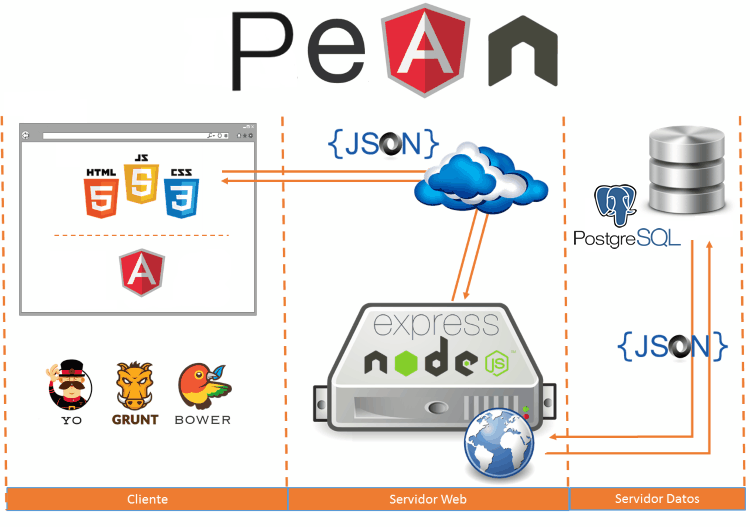
\includegraphics[width=0.9\textwidth]{images/01-stack.png}
	\medskip
	\caption{Diagrama representativo del stack y las \\ tecnologías que la componen.}
	\medskip
\end{figure}
\bigskip


% CAPITULO X
\subsection{Frontend}

	El Frontend es la división representada por el cliente, el cual, en nuestro caso está protagonizado por el navegador utilizado por este. Para esta parte se utilizarán las siguientes tecnologías:

	\begin{itemize}
	\renewcommand{\labelitemi}{\scriptsize\tiny$\blacksquare$} 
	\itemsep=7pt \topsep=0pt \partopsep=0pt \parskip=0pt \parsep=0pt

		\item \textit{HTML5}: Es un lenguaje de marcado para la elaboración de sitios web. Es un estandar que sirve de referencia para construir sitios webs mediante una estructura básica que define la semántica de los datos que lo componen. Dichos datos pueden ser texto, imágenes, videos, entre otros.
		
		\item \textit{CSS3}: Las hojas de estilo nos permiten definir de manera eficiente la representación de nuestras páginas en cuanto al diseño y visualización de estas. Permiten definir estructuras guiadas por el futuro atractivo proyectado para nuestras webs, aplicar colores, animaciones, formas, distribuciones, entre otras cosas.

		\item \textit{JS}: es un lenguaje de programación que permite a los desarrolladores crear acciones y capturar eventos iniciados por los usuarios en sus sitios webs. Es decir, JavaScript es un lenguaje utilizado para crear pequeños programas que luego son insertados en una página web y en programas más grandes, orientados a objetos mucho más complejos. Con JS podemos crear diferentes efectos e interactuar de manera dinámica con los usuarios.
		
		\item \textit{AngularJS}\footnote{\url{http://www..com/}}: .
		
		\item \textit{YEOMAN}\footnote{\url{http://www..com/}}: .

		\item \textit{Grunt}\footnote{\url{http://www..com/}}: .

		\item \textit{Bower}\footnote{\url{http://www..com/}}: .

	\end{itemize}
	
\newpage


% CAPITULO X
\section{Backend}
	El backend es donde corre la aplicaci\'{o}n real, donde se encuentra la l\'{o}gica del programa y donde se encuentran programadas las reglas del negocio, as\'{i} como tambi\'{e}n las conexiones con las bases de datos y API's.\\
	
	
Para el servidor en donde procesaremos todas las solicitudes, hemos optado por utilizar Node.js, un entorno de ejecuci\'{o}n de aplicaciones multiplataforma que utiliza javascript. Es decir, estamos utilizando javascript del lado del servidor. Utilizar Node.js nos proporciona un rendimiento y una escalabilidad muy elevadas dada la arquitectura orientada a eventos y APIs no bloqueantes que provee. La aplicación hecha en Node.js es la que actuar\'{a} como Servidor web.\\

Para el almacenamiento de los datos, necesitamos por un lado tener cierta estructura para el registro de usuarios. Sin embargo, tambi\'{e}n vamos a tener que almacenar datos que carecen de una estructura definida, tales como pueden ser las distintas m\'{e}tricas obtenidas de las diferentes redes sociales, las cuales var\'{i}an en su formato, por lo que vamos a requerir cierta flexibilidad, en nuestro caso, para guardar datos con formato JSON.\\
Por esta raz\'{o}n es que hemos elegido utilizar PostgreSQL, un motor de base de datos h\'{i}brido en el que conviven caracter\'{i}sticas de las bases de datos relacionales y no relacionales.\\

Entonces, las ventajas que pudimos ver en usar PostgreSQL como motor de bases de datos son:

\begin{itemize}

\item La posibilidad de utilizar bases de datos no relacionales, las cuales son f\'{a}cilmente escalables, esto quiere decir, que pueden crecer mucho sin necesidad de realizar cambios a su estructura, una caracter\'{i}stica de importancia para el volumen de datos que manejamos. 

\item El ahorro de ancho de banda.

\item Las operaciones que podemos realizar sobre los datos almacenados (en formato JSONB), tales como b\'{u}squedas indexadas, las cuales son mucho m\'{a}s r\'{a}pidas que en bases de datos relacionales. Esta caracter\'{i}stica es relevante ya que para nuestro negocio la performance es de vital importancia.

\item  Y por si no fuera poco, PostgreSQL es muy escalable horizontalmente, lo que significa que ante la necesidad de ampliar el procesamiento, es posible agregar m\'{a}s equipos que distribuyan la carga.

\end{itemize}


Es claro que hemos usado muchos frameworks que conviven entre s\'{i}. Estos nos facilitan el desarrollo al contar con soluciones previamente codificadas a problemas conocidos y de uso diario. Por lo tanto, estamos ahorrando tiempo, y por ende, dinero, d\'{a}ndonos lugar a plasmar nuestra idea sobre bases s\'{o}lidas en forma veloz. \\


En resumen, se utilizar\'{a}n:
	
	\begin{itemize}
		\item \textbf{NodeJS} para el servidor 
		\item \textbf{API's de redes sociales} para provisionamiento de datos: Facebook, Twitter, Google+, etc.
		\item \textbf{PostgreSQL} como motor de base de datos.
		\item \textbf{PgAdmin III} como administrador de esquemas de base de datos.
		
	\end{itemize}
	
\newpage



% CAPITULO X
\section{Integración con redes sociales}

En orden de obtener los datos requeridos se utilizarán las API's proveidas por las distintas redes sociales. En particular, se usarán:

\subsection{Facebook}


	\subparagraph*{Graph API\footnote{Documentaci\'{o}n en \url{https://developers.facebook.com/docs/graph-api}}}
	
	Esta API permite leer y escribir en el grafo social de Facebook.
	Permite encontrar relaciones, obtener y emitir publicaciones, compartir contenido, consultar por likes en publicaciones, etc.\\
	
	Aqu\'{i} se muestran algunos ejemplos de su uso:\\
	
	\begin{itemize}
  		\item Obtener c\'{a}ntidad de likes a la p\'{a}gina: \texttt{id\_pagina?fields=likes}
  		\item Obtener publicaciones: \texttt{id\_pagina?fields=feed}
  		\item Obtener likes de una publicaci\'{o}n: \texttt{id\_post/likes}
  		\item Obtener comentarios (de cualquier objeto que pueda tener comentarios): \texttt{id\_objeto/comments}
  		\item Obtener si a un usuario le gusta una p\'{a}gina: \texttt{id\_usuario/likes/id\_pagina}
  		\item etc...
	\end{itemize}
	
	Esta API devuelve datos en formato de objeto JSON, a partir del cual se pueden extraer los de inter\'{e}s facilmente.
	
	

	\subparagraph*{Insights API\footnote{Documentaci\'{o}n en \url{https://developers.facebook.com/docs/graph-api/reference/v2.4/insights}}}

	Esta API permite obtener datos a partir de m\'{e}tricas definidas en la misma sobre la actividad de una p\'{a}gina, sobre el contenido publicado en ella y sobre el contenido que hace referencia a ella en otros entornos de facebook.
	Para poder utilizar esta API, la p\'{a}gina de facebook debe tener al menos 30 likes.
	Esta herramienta nos brinda casi todos los datos que necesitamos (y algunos m\'{a}s que no habiamos tenido en cuenta):
	
	Aqu\'{i} se muestran algunos ejemplos de su uso:\\

	\begin{itemize}
  		\item Obtener el n\'{u}mero de personas que comparten historias acerca de una p\'{u}gina (personas están hablando de esto). Estas historias incluyen likes a la p\'{a}gina , publicar en el muro de la misma, dar like, comentar o compartir en uno de las publicaciones de la p\'{a}gina\; responder a una pregunta publicada, responder asistencia a un evento, menciones de la p\'{a}gina, phototagging de la p\'{a}gina, etc:\\ 
  		\texttt{id\_pagina/insights/page\_storytellers}

  		\item Obtener personas que estan hablando de la p\'{a}gina por edad y g\'{e}nero:\\
  		\texttt{id\_pagina/insights/page\_storytellers\_by\_age\_gender}

  		\item Obtener cantiadad de historias acerca de una publicaci\'{o}n:\\
  		\texttt{id\_post/insights/post\_stories}

  		\item Obtener cantidad de usuarios comprometidos con una p\'{a}gina. El estar comprometido incluye realizar clicks en dicha p\'{a}gina:\\
  		\texttt{id\_pagina/insights/page\_engaged\_users}

  		\item Obtener cantidad de usuarios que le gusta una p\'{a}gina por ciudad:\\
  		\texttt{id\_pagina/insights/page\_fans\_city}

  		\item etc...
	\end{itemize}
	
	Esta API devuelve datos en formato de objeto JSON, a partir del cual se pueden extraer los de inter\'{e}s facilmente.


	\subparagraph*{Otras API's}
	Existen otras API's proveidas por Facebook, aunque su acceso es restringido a usuarios con ciertos permisos. Para tener tales permisos se debe enviar una solicitud a Facebook para el uso de estas API's.
	Estas son:
	\begin{itemize}
		\item \textbf{Public Feed API:} Permite mostrar en tiempo real la actividad p\'{u}blica relacionada a un cierto t\'{e}rmino (tal como “Messi” o “Grammys”). Solo posts p\'{u}blicos de p\'{a}ginas y usuarios importantes con la opci\'{o}n “seguir” activada podr\'{a}n ser mostrados. Esto permite saber las opiniones del p\'{u}blico acerca de un cierto tema.
		\item \textbf{Keyword Insights API:} Permite saber la cantidad total de menciones de un t\'{e}rmino en una cierta ventana de tiempo, haciendo m\'{a}s f\'{a}cil a nuevas organizaciones ver cuanta gente estaba hablando acerca de un evento antes, durante o despu\'{e}s del mismo. Tambi\'{e}n permite mostrar cifras an\'{o}nimas con filtros como g\'{e}nero, edad y localizaci\'{o}n. Esto permite saber qu\'{e} es trending topic, entre otras cosas.
	\end{itemize}
	
\bigskip

\subsection{Twitter}
Las APIs disponibles para acceder a contenido de twitter son:
\begin{itemize}
	\item \textbf{Public API:} Esta API provee acceso a contenidos de Twitter para lectura y escritura. Publicar un nuevo tweet, obtener datos del perfil de una persona y de seguidores, y mucho mas.
	\textbf{Streaming API:} Permite acceso a datos de Twitter en tiempo real, tal como la Keywords Insights API y la Public Feed API de Facebook.
\end{itemize}


Se necesita registrar la aplicaci\'{o}n que se va a utilizar en Twitter\footnote{\url{https://apps.twitter.com/}}. Una vez registrada se podr\'{a}n ver los datos necesarios para poder acceder a la API Rest que brinda Twitter.

	\subparagraph*{Public API\footnote{\url{https://dev.twitter.com/rest/public}}}
	Algunos ejemplos de su uso pueden ser los siguientes:

	\begin{itemize}
		\item Obtener retweets de la propia cuenta:  \\
		\texttt{/statuses/retweets\_of\_me}

		\item Obtener lista de favoritos: \\
		\texttt{/favorites/list.json?parametros}

		\item Obtener la lista de seguidores:\\
		\texttt{/followers/list}
	
		\item Obtener cantidad de hashtags mencionados relacionados a cierto tema:\\
		\texttt{/search\#tema\_buscado}
	
		\item etc...

	\end{itemize}	 

\bigskip

\subsection{Google+}

	\subparagraph*{Page API}
	Google brinda una API para manejo de páginas de Google+, obtener datos de seguidores, publicaciones y publicar contenido. Esta API es la \textbf{Page API} y debe enviarse una solicitud a Google para poder utilizarla.
	\subparagraph*{Analytics APIs}
Además Google provee del servicio de Google Analytics muy similar al servicio de Insights de Facebook. Este servicio tiene disponibles las siguientes APIs para consulta de datos enriquecidos y métricas:
	\begin{itemize}
		\item \textbf{Real Time Reporting API} 
		\item \textbf{Core Reporting API}
	\end{itemize}





\newpage


% CAPITULO X
\section{Casos de Uso}

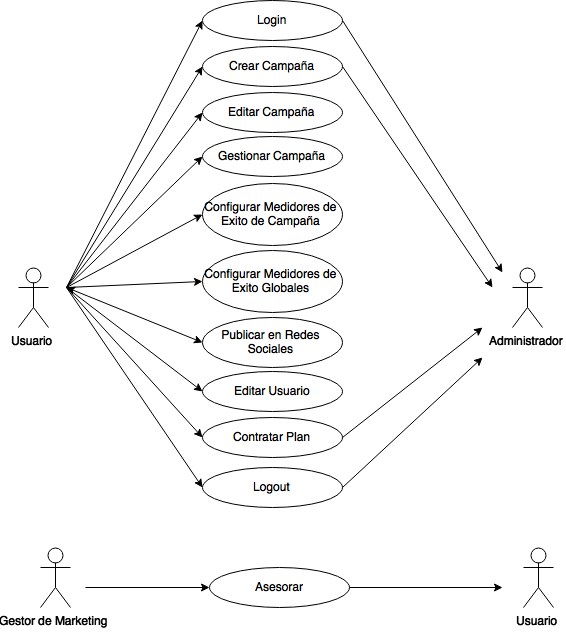
\includegraphics[width=0.9\textwidth]{images/casosDeUso.png}

\newpage



\section{Modelo de datos}

El modelo de datos consistir\'{a} en el siguiente esquema:
	
% Imagen 
\begin{figure}[H]
	\centering
	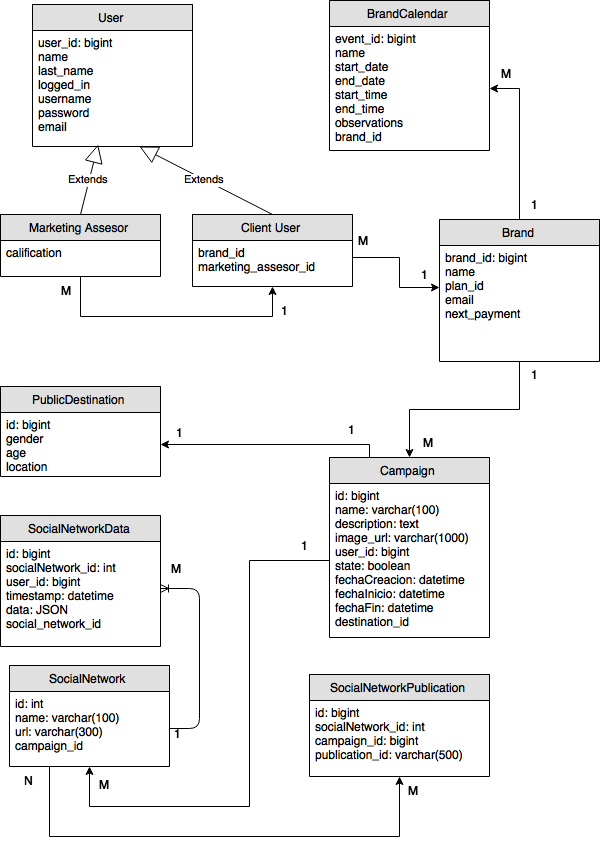
\includegraphics[width=0.9\textwidth]{images/weepo-01.png}
	\medskip
	\caption{Tablas de la base de datos.}
	\medskip
\end{figure}	
	
\newpage


% CAPITULO X
\section{Puesta en producción}

El desarrollo es muy importante, pero al comenzarlo es crítico tener en mente cómo va a ser la puesta en producción, es decir, dónde vamos a alojar nuestra aplicación. Debemos estar preparados para un posible éxito, y esto significa que el hosting que elijamos debe ser capaz de darnos la oportunidad de escalar los servicios para lograr un rendimiento sostenido.\\
Por suerte son varias las opciones entre las cuales podemos elegir, entre las más conocidas AWS, Google Cloud Platform y Microsoft Azure. Pero para empezar nos decidimos por OpenShift ya que proveen de un plan gratuito con posibilidad de habilitar planes pagos en forma automática y escalabilidad instantánea de nuestra aplicación cuando sea oportuno, además poder apuntar en forma gratuita el dominio del sitio web de Weepo.

\newpage




%
% CAPITULO Y
%
\chapter{Demo del servicio}


% CAPITULO Y
\section{Alcance}

En esta secci\'{o}n se mostrar\'{a}n algunas pantallas que intentan ilustrar algunas de los puntos de acceso del usuario y las funcionalidades b\'{a}sicas de la herramienta.
\bigskip


% CAPITULO Y
\section{Capturas de pantalla}

\subsection{P\'{a}gina de inicio}


\includegraphics[width=0.9\textwidth]{images/index.png}
\medskip

\subsection{Administraci\'{o}n de Campañas}

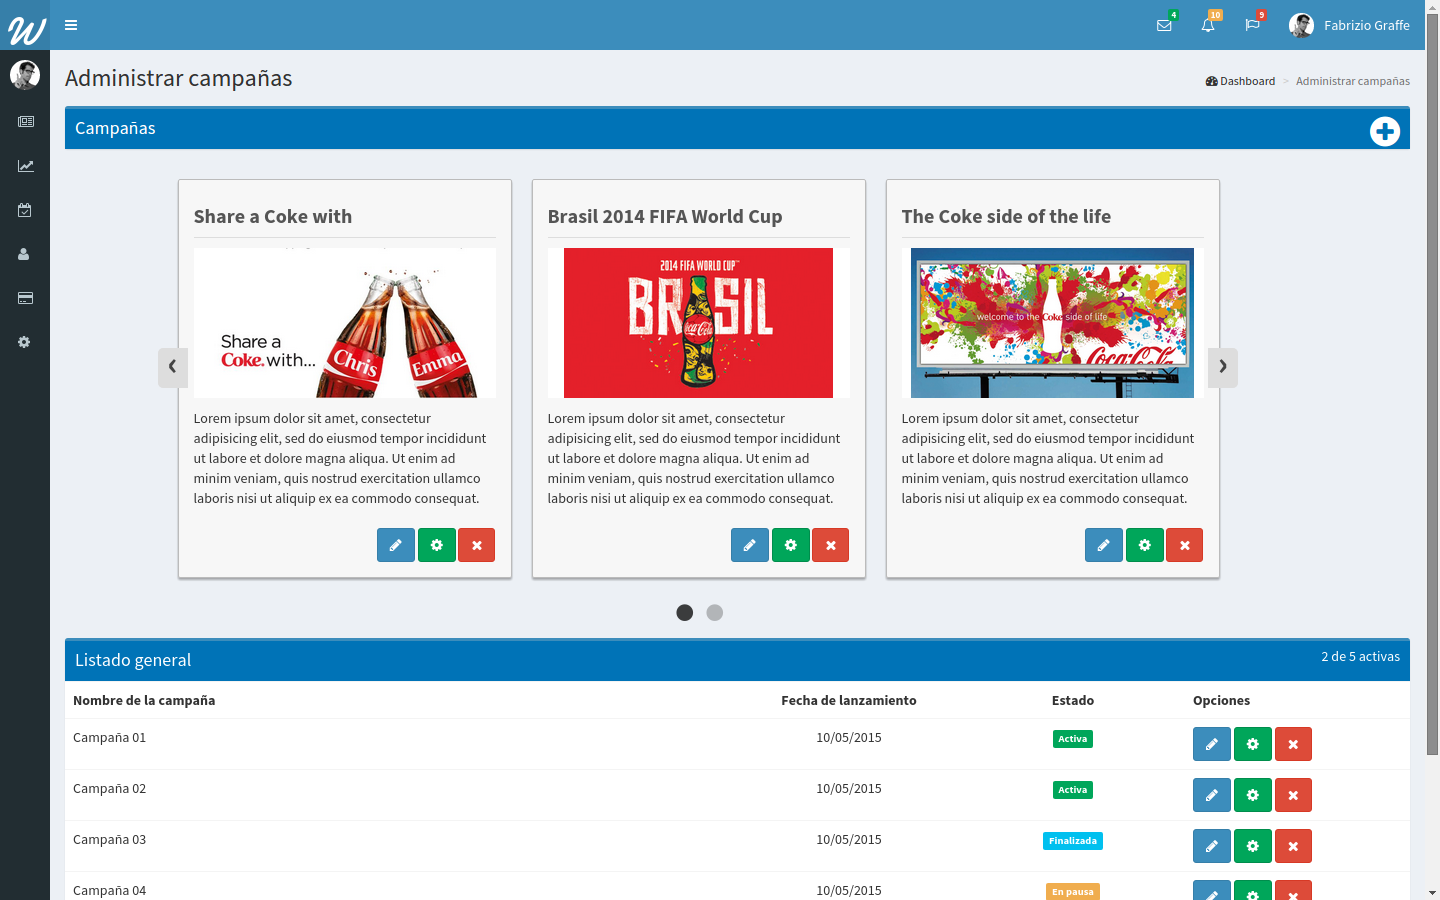
\includegraphics[width=0.9\textwidth]{images/adminCampanias.png}

\medskip
\subsection{Informaci\'{o}n General}

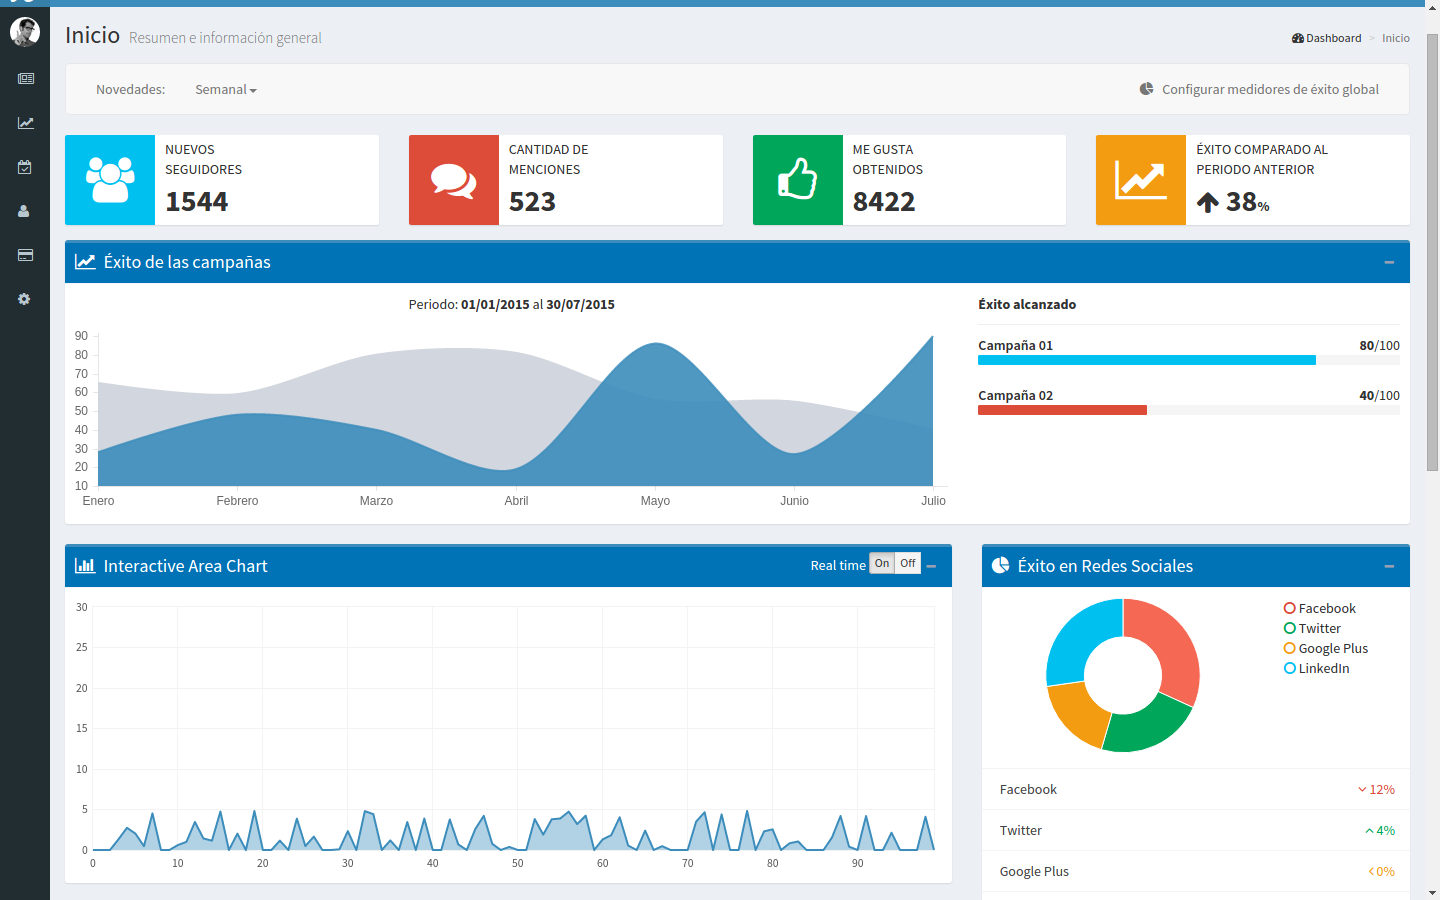
\includegraphics[width=0.9\textwidth]{images/InfoGral.png}

\medskip
\subsection{Administraci\'{o}n de Eventos}

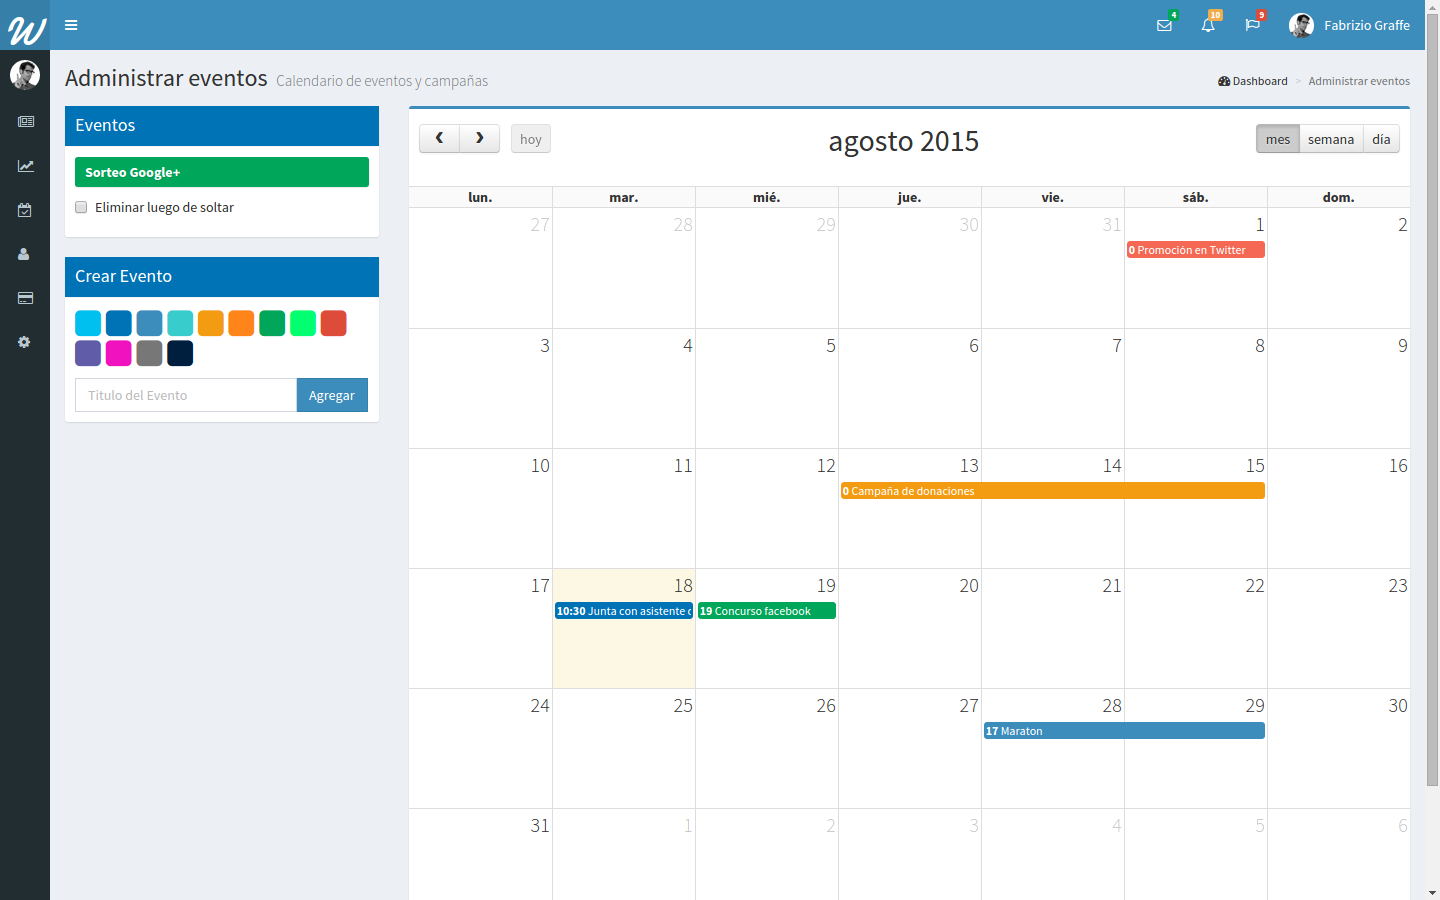
\includegraphics[width=0.9\textwidth]{images/adminEventos.png}

\medskip
\subsection{Precios}

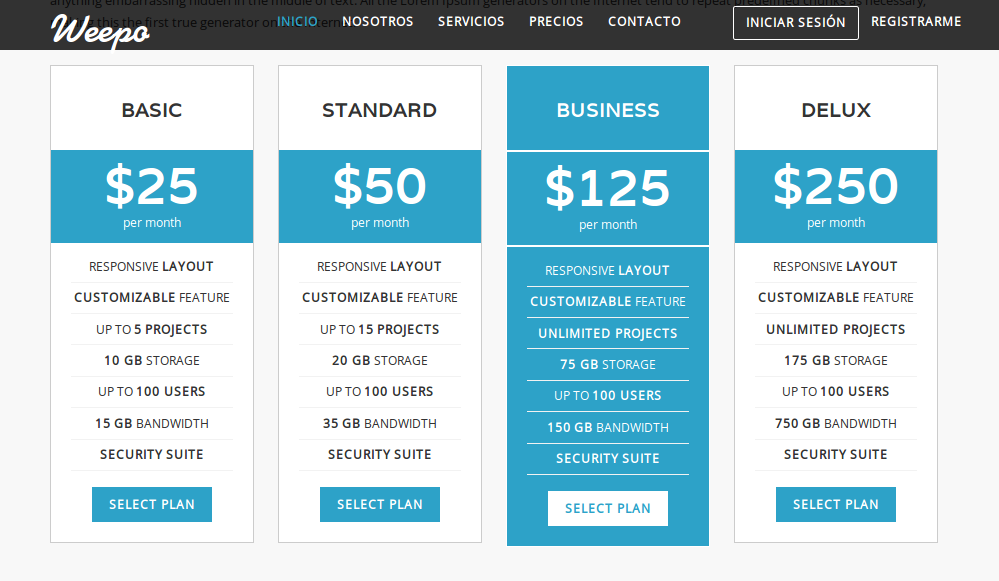
\includegraphics[width=0.9\textwidth]{images/business.png}

\medskip
\subsection{Asesores de Marketing}

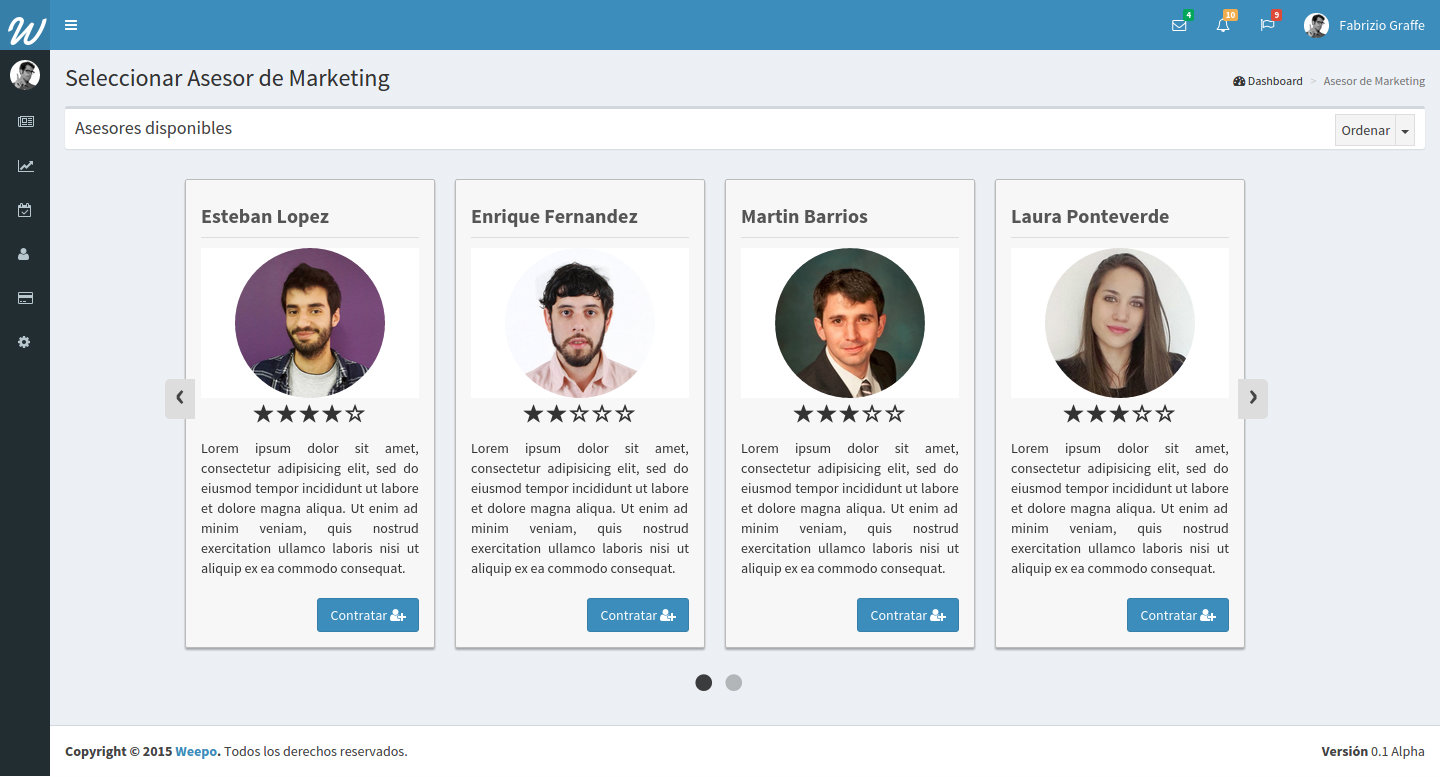
\includegraphics[width=0.9\textwidth]{images/asesorDeMarketing.jpg}



\bigskip



% %
% % CAPITULO 1
% %
% \chapter{Enunciado}



% % CAPITULO 1
% % Implementación pedida
% \section{Implementación pedida}

% En esta segunda iteración se pide extender el modelo de dominio realizado en la \textit{primera iteración}\footnote{Se hará referencia al informe corresponiente a la primera iteración, el cual puede descargarse desde \url{http://www.google.com/+/learnmore/hangouts/?hl=es-419}}, de manera de soportar los requerimientos que se detallarán en los apartados siguientes.
% \bigskip



% % CAPITULO 1
% % El laberinto y sus bolitas
% \subsection{El laberinto y sus bolitas}

% El laberinto define: la distribución de lugares válidos de transito en
% donde en cada una de estas posiciones hay bolitas (o bolones) y los lugares posibles por donde se desplazan los fantasmas y el pacman.
% \par
% Tiene definido también la posición de inicio del pacman y el lugar de donde salen los fantasmas (al comienzo y cuando pasan de estado muerto a estado cazador).
% \par
% Las bolitas y los bolones son comidos únicamente por el pacman.
% \par
% Cuando un bolón es comido, todos los fantasmas que están en estado cazador son convertidos a presa (por un intervalo x de tiempo) y todos los que son presa permanecen presa (por el mismo intervalo x de tiempo).
% \par
% Se pide modelar el laberinto del pacman (con sus N bolones y sus portales)
% \par
% El laberinto debe instanciarse a partir de un archivo, donde se indican:

% \begin{itemize}
% \renewcommand{\labelitemi}{\scriptsize\tiny$\blacksquare$} 
% \itemsep=2pt \topsep=0pt \partopsep=0pt \parskip=0pt \parsep=0pt

% 	\item Las conexiones entre los eslabones del laberinto.

% 	\item Qué eslabones contienen bolitas o bolones.

% \end{itemize}	
% \smallskip

% El formato del archivo de definición de laberintos esta definido, descargar el campus.
% \par
% No se pide modelar en esta iteración el manejo de partidas con niveles, ni tampoco de puntajes por bolita comida.
% \par
% Dado que no hay interfaz gráfica en esta iteración, se desea tener un  mecanismo de notificación ante cada iteración, intervalo o tick del estado del juego. Dicha notificación debe ser serializada en archivos xml con el estado de cada iteración del juego.
% \par
% Para ello, ante cada iteración o tick del juego, se solicita leer de un archivo el movimiento elegido para el pacman, realizar los movimientos correspondientes y luego serializar a un xml el estado del juego para ese tick. El formato solicitado para la serialización tanto para el movimiento elegido del pacman, como al del estado del juego, ya estan definidos y se descargaran del campus.
% \bigskip


% % CAPITULO 1
% % El pacman
% \subsection{El Pacman}

% El mismo recibirá las órdenes del usuario para moverse en las cuatro direcciones. El pacman siempre tiene una velocidad de 2 x <Velocidad del fantasma en estado normal>. (Los fantasmas tienen la velocidad minima 1 en estado normal, 1,5 en estado molesto y 2 en estado furioso).
% \par
% Cuando el pacman come un fantasma cazador (o es cazado por un fantasma) muere.
% \bigskip


% % CAPITULO 1
% % Comportamiento autómata de los fantasmas
% \subsection{Comportamiento autómata de los fantasmas}

% Los fantasmas en estado cazador pueden desplazarse al menos en alguno de los siguientes cuatro criterios de inteligencia:

% \begin{itemize}
% \renewcommand{\labelitemi}{\scriptsize\tiny$\blacksquare$} 
% \itemsep=2pt \topsep=0pt \partopsep=0pt \parskip=0pt \parsep=0pt

% 	\item \textit{Zonzo}: Se mueve aleatoriamente, solamente se lanza a comer al pacman si este se encuentra a N1 (a cuatro casilleros seguidos por ejemplo) lugares de distancia, si este se escapa a mas de N1 lugares continúa moviéndose aleatoriamente;

% 	\item \textit{Perezoso}: Se mueve aleatoriamente, solamente se lanza a comer al pacman si este se encuentra a N2 (ocho por ej) lugares de distancia;

% 	\item \textit{Buscador}: Se mueve aleatoriamente, si el pacman se encuentra a N3 lugares de distancia lo persigue. Si el pacman se escapa a más de N3 (diez por ej) lugares de distancia el fantasma buscador va hacia la última posición donde lo vio (no se mueve de manera aleatoria) y si en el camino lo ve, se dirige hacia esa posición;

% 	\item \textit{Buscador temperamental}: Es igual al buscador anterior, pero si el fantasma incrementa su nivel de ira incrementa en X la visión (inicialmente tiene una visión de N4 lugares(12). Si se reinicia el nivel de ira, entonces también se reinicia la visión).

% \end{itemize}	
% \smallskip

% El movimiento aleatorio mencionado anteriormente tiene que cumplir con los siguientes requerimientos:

% \begin{itemize}
% \renewcommand{\labelitemi}{\scriptsize\tiny$\blacksquare$} 
% \itemsep=2pt \topsep=0pt \partopsep=0pt \parskip=0pt \parsep=0pt

% 	\item Una vez que entra a un canal del laberinto, sigue hasta llegar a un cruce o bifurcación, recién ahí vuelve a decidir hacia donde ir. Y no es opción regresar por donde vino, a menos que sea un canal sin salida;

% 	\item A la llegada de un cruce si no sabe a donde ir, dado su visión, entonces define aleatoriamente que camino tomar;

% 	\item Siempre se mueven, una vez entrado a un canal sigue hasta salir del mismo, al llegar a un cruce decide a donde ir, es decir nunca están quietos;

% \end{itemize}	
% \smallskip

% El fantasma en estado presa debe alejarse del pacman, es decir que se debe moverse según se describió pero alejándose en los casos que antes se acercaba al pacman.
% \bigskip



% % CAPITULO 1
% % Test unitarios
% \subsection{Test unitarios}

% Se piden un set de test unitarios sobre el modelo de dominio descrito en el apartado 1.1.1
% \par
% El set de test unitarios que se desarrolle debe representar un código valioso, debe motivar al equipo de trabajo a mantenerlo en el tiempo por la utilidad que brinda. Debe seguir las buenas prácticas de implementación de test unitarios.
% \par
% Se debe contemplar un conjunto amplio y abarcativo de casos de prueba sobre el modelo de dominio.
% \bigskip


% % CAPITULO 1
% % Aclaraciones sobre la implementación
% \section{Aclaraciones sobre la implementación}

% Quedan fuera de la presente iteración los siguientes requerimientos:

% \begin{itemize}
% \renewcommand{\labelitemi}{\scriptsize\tiny$\blacksquare$} 
% \itemsep=2pt \topsep=0pt \partopsep=0pt \parskip=0pt \parsep=0pt

% 	\item Interfaz gráfica del pacman.

% 	\item Sistema de partidas: Jugadores y turnos, vidas y puntajes, nuevos laberintos. (El juego arranca en estado inicializado según el archivo que lo describe, y termina al morir el pacman o al comer todas las bolitas).

% 	\item Lógica de cómo un fantasma muerto, regresa al inicio (como se desplazaría de muerto a su lugar de inicio). Directamente desaparece y aparece cuando revive del punto de inicio.

% 	\item Otras estrategias de los fantasmas cazadores de cómo atacar al pacman (si eligen el camino mas corto o más largo, si lo encierran en grupo, etc).

% 	\item En caso de tomar una decisión de implementación que esté fuera del alcance descripto, esta no debe contradecir ningún requerimiento pedido y se debe enunciar en el informe la hipótesis que la justifique, las mismas deben validarse con el ayudante.

% \end{itemize}	
% \bigskip




% %
% % CAPITULO 2
% %
% \chapter{Diseño del dominio}

% De aquí en adelante iniciaremos la búsqueda de una solución en la que se tendrá como objetivo aplicar criterios que nos permitan llegar a buen diseño, es decir, obtener una estructura robusta que carezca de rigidez, fragilidad e inmobilidad. 
% \par
% Con el fin de conducir el diseño a una buena representación del dominio manteniendo la meta propuesta es que se aplicarán los principios SOLID. En los próximos apartados iremos profundizando sobre la extensión del modelo exponiendo además los principios SOLID que habremos de aplicar.
% \bigskip\bigskip

% % Imagen 
% \begin{figure}[H]
% 	\centering
% 	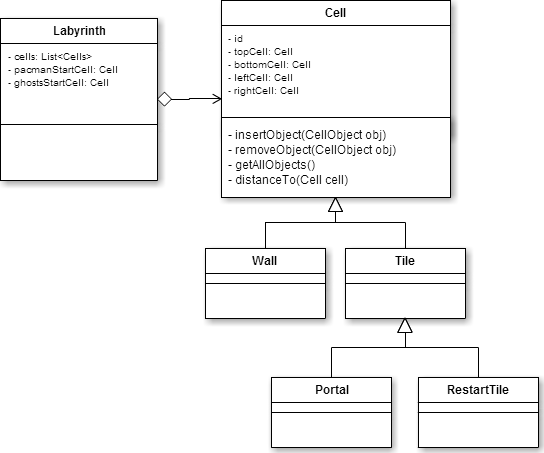
\includegraphics[width=0.7\textwidth]{images/generalDiagram01.png}
% 	\medskip
% 	\caption{Diagrama de clases con enfoque sobre \\ las celdas del laberinto.}
% 	\medskip
% \end{figure}
% \bigskip


% % CAPITULO 2
% % Celdas
% \section{Celdas}

% Esta entidad surge de la necesidad de expresar en nuestro modelo un concepto de posición dentro del laberinto del pacman. Esta noción comienza obligatoriamente por querer darle valor y existencia a esa posición, y se luce como una entidad abstracta dada su generalidad.
% \par
% La necesidad real fue inicialmente la idea de baldosa, que representa el camino por el cual puede circular tanto el pacman como los fantasmas. De este se desprende otra idea, que es la de querer representar de alguna manera por donde no pueden circular estos objetos que se desplazan. Pero como hablamos, se tratan de elementos dentro del laberinto demasiado concretos y en cierta forma son bastante semejantes, como conclusión al observar esto se decidio generalizarlos de manera que se obtuvo el concepto de celda. El diagrama de clases que expresa esta última idea puede observarse en la \textit{Imagen 2.1}.
% \bigskip


% % CAPITULO 2
% % Objetos de celda
% \subsection{Objetos de celda}

% Teniendo el concepto de celda y agregando la clara noción de que cada celda contendría objetos en concepción de ``distintos objetos se encuentran en determinada celda'' incursionamos en un gran debate que radicaba en comprender qué eran esos objetos que contenía mas allá de saber cuales eran (pacman, fantasma, bolita, bolon).
% \par
% Para esto se comenzó pensando en que deberían tener en común estos elementos, y particularmente detectamos la necesidad de que sean objetos posicionables lo cual define que el objeto sabe colocarse en una celda. Por otro lado se detectó que tiene sentido que estos objetos colisionen entre sí. Y por ultimo, como es el corazón del juego, es indispensable que todos los objetos sean comibles ya que si no fuera así no estaríamos hablando del pacman.
% \par
% De esta manera surgió la entidad \textit{CellObject} para identificar cualquier elemento contenido en una celda, la cual es una entidad abstracta que representa cualquier tipo de objeto posible en el mismo permitiendo gran desacoplamiento y extensibilidad. En la \textit{Imagen 2.2} se puede observar el diagrama de clases de este diseño planteado.
% \bigskip\medskip

% % Imagen 
% \begin{figure}[H]
% 	\centering
% 	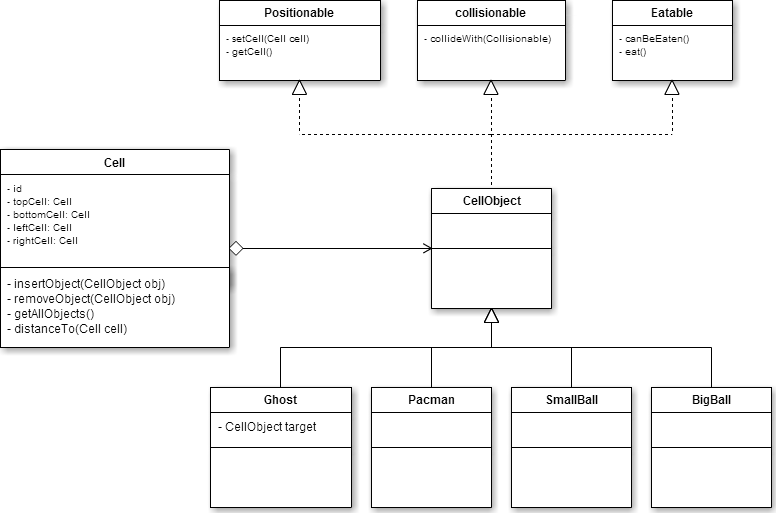
\includegraphics[width=0.90\textwidth]{images/generalDiagram02.png}
% 	\medskip
% 	\caption{Diagrama de clases con enfoque sobre \\ los objetos de las celdas del laberinto.}
% 	\medskip
% \end{figure}
% \bigskip


% % CAPITULO 2
% % Notificaciones de objetos comibles
% \section{Notificaciones de objetos comibles}

% La idea de comible ya había surgido anteriormente en la primer iteración del proyecto, pero no se había profundizado en gran medida. En esta nueva etapa se logró captar su esencia semántica y simplificar su implementación dejando en claro que ``\textit{cuando un objeto, tanto pacman, fantasma, bolita o bolón, es comido simplemente este muere pero no necesariamente sabe que pasa cuando él muere}''.
% \par
% La observación anterior nos permitió pensar como uno de esos objetos y así llegar a una conclusión. En la mayoria de los casos un objeto no necesitaría saber que pasa luego de que ``muere'' pero por el contrario es muy problable que alguien pueda estar interesado en ello, de manera que incorporamos la idea de observador de objetos comibles.
% \par
% Los observadores de objetos comibles básicamente serían objetos que estarían interesados en saber cuándo un objeto en particular fue comido y así poder tomar alguna decisión o interacción necesaria. En la \textit{Imagen 2.3} puede visualizarse el diagrama de clases que representa el concepto recién explicado.
% \bigskip\bigskip

% % Imagen 
% \begin{figure}[H]
% 	\centering
% 	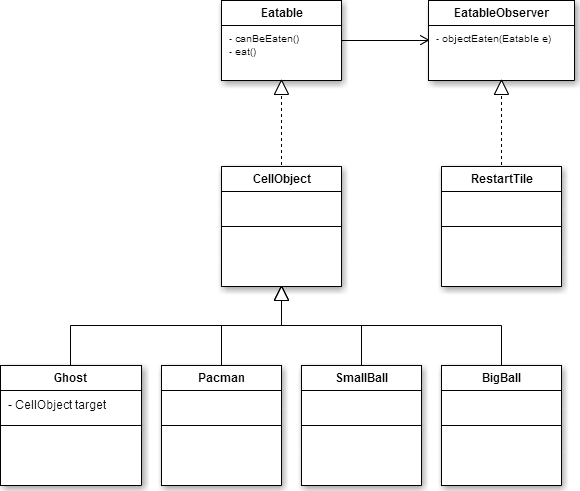
\includegraphics[width=0.80\textwidth]{images/generalDiagram03.png}
% 	\medskip
% 	\caption{Diagrama de clases con enfoque sobre \\ la clase observadora de comibles.}
% 	\medskip
% \end{figure}
% \bigskip


% % CAPITULO 2
% % Baldozas de inicio
% \subsection{Baldozas de inicio}

% Para el inicio de los fantasmas como así también del pacman, se le indica al laberinto dichas celdas a las cuales se les agregan estos objetos tal como corresponda.
% \par
% De lo anterior, dado el alcance de la iteración, cuando un fantasma muere debe volver a su posición de inicio. Para resolver esta cuestión se optó por implementar un tipo de baldosa cuya función es ser la posición de reinicio de cualquier objeto comido que se encuentre observando. Esto se implementó fácilmente utilizando la interfaz \textit{EatableObserver} sobre cada uno de los fantasmas, y de esta manera cada vez que los fantasmas son comidos por el pacman estos automaticamente se mueven a su posición de reinicio.
% \bigskip


% % CAPITULO 2
% % Muerte de los fantasmas
% \subsection{Muerte de los fantasmas}

% Cuando el fantasma se encuentra en estado presa puede llegar a ser comido por el pacman. Si eso sucediera, sería necesario cambiar su estado y reubicarlo en la celda de inicio que le corresponde. Dado que que dicha celda solo es conocida por el laberinto, se presenta la necesidad de comunicar el evento ocurrido. 
% \par
% Por ello se utilizó una interfaz como \textit{EatableObserver} que pueda ser implementada por aquella clase que sepa como reubicar al fantasma. Así, cada \textit{CellObject} puede tener una serie de observadores, cuyo método correspondiente es invocado cuando el antedicho \textit{CellObject} es comido.
% \par
% En este caso, la clase que implementa \textit{EatableObserver} para el fantasma es \textit{RestartTile}. De este modo, cuando el fantasma es comido, se le avisa al mismo para que cambie su estado a muerto, pero también a la celda de reinicio, que al tener un comportamiento especial, puede reubicar al \textit{CellObject} en sí misma.
% \bigskip


% % CAPITULO 2
% % Muerte del pacman
% \subsection{Muerte del pacman}

% Al igual que para los fantasmas, también debe existir un método para comunicar la muerte del pacman. Al ser este también un \textit{CellObject}, tiene una lista de observadores a los cuales se avisa en caso de suceder este evento. Los observadores pueden ser, nuevamente, de cualquier clase que implemente \textit{EatableObserver}. 
% \par
% En este caso es el laberinto mismo quien controlará este suceso. De modo que al comer al pacman este avisa a su observador, el laberinto, el cual a su vez realiza las acciones correspondientes, ya sea terminar el juego, descontar una vida o reubicar al pacman.
% \bigskip


% % CAPITULO 2
% % Bolitas y Bolones comidos
% \subsection{Bolitas y bolones comidos}

% La solución propuesta para el manejo de las bolitas y los bolones se centró en dos aspectos o cuestiones: \textit{¿Quien se encarga de sacarlo de su celda? ¿Quien se encarga de efectuar el alcance de que haya sido comido (puntaje o convertir a los fantasmas)?}
% \par
% Luego de debatir la responsabilidad de estos aspectos consideramos indicado dejar que la misma bolita o el bolón se encargue de quitarse a si mismo de su celda luego de ser comido. Pero no fue así para su accionar luego de ser comido, para este caso nos pareció prudente que el laberinto se encargue de observar cuando alguno de estos objetos es comido y asi poder actuar correctamente.
% \bigskip


% % CAPITULO 2
% % Comportamiento de los fantasmas
% \section{Comportamiento de los fantasmas}

% Los fantasmas son entidades que comparten cualidades y comportamientos comunes, más allá de las diferencias que se hallan entre unos y otros. Poseen una presa, un estado, sea este cazador, presa o muerto, y un rango de visión dentro del cual pueden ver a la presa. Todos estos deben ser identificados como atributos o propiedades de dicha entidad. Por otro lado, tienen comportamientos compartidos, sean estos la posibilidad de cambiar de estado, de moverse, perseguir a la presa o huir de ella, comerla o ser comidos.
% \par
% Dado que, sin importar cual sea su inteligencia, todos son fantasmas, la mejor forma de representar los distintos tipos de fantasmas es mediante un mecanismo de herencia. De este modo, las diferencias que hay entre ellos, como el rango de visión, pueden ser modificadas haciendo solo leves ajustes.
% \par
% Se plantean cuatro tipos de inteligencia, sin embargo la cuarta, el buscador temperamental es, básicamente, un fantasma buscador. Por lo tanto, nuevamente se plantea una relación de herencia entre ellos. Entonces, la estructura de clases de los fantasmas quedaría como en la \textit{Imagen 2.1}.
% \bigskip


% % Imagen 
% \begin{figure}[H]
% 	\centering
% 	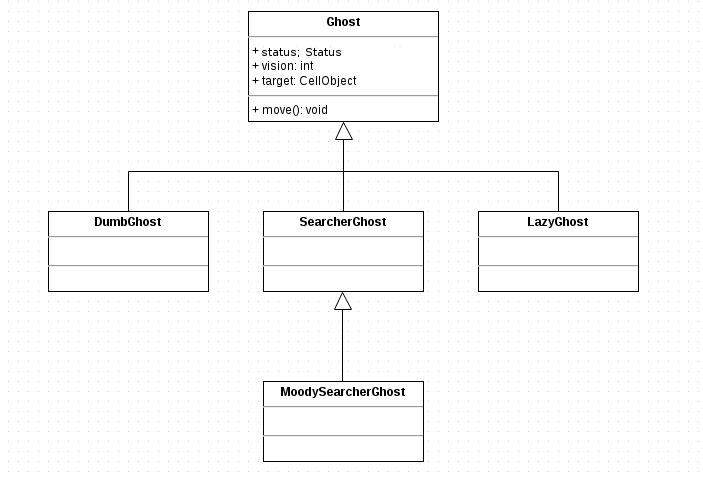
\includegraphics[width=0.86\textwidth]{images/ghostDiagram.png}
% 	\caption{Diagrama de clases con enfoque sobre \\ los comportamientos de los fantasmas.}
% 	\medskip
% \end{figure}
% \bigskip


% Los fantasmas tienen como comportamiento común el poder moverse de forma relativa a su presa o aleatoria, dependiendo de si esta se encuentra dentro de su rango de visión o no. Si se encuentran en estado cazador procuran acercarse a su presa y si están siendo perseguidos, se alejan de ella. Por lo que este comportamiento es genérico para todos sus tipos. Solo el buscador puede moverse con otro criterio, de modo que él mismo deberá redefinir su movimiento. Sucede algo similar con el aumento en la vision del buscador temperamental, quien deberá corroborar a medida que pase el tiempo si ha variado su agresividad. De este modo, lo que debería redefinir cada tipo de fantasma sería, principalmente, su rango de visión.



% %
% % CAPITULO 3
% %
% \chapter{Control y serialización}

% Para la presente iteración, como ya se ha remarcado en el \textit{Capítulo 1}, ha quedado fuera del alcance todo aquello referente al sistema de partidas, es decir, los jugadores, turnos, vidas y puntajes, como así también los distintos laberintos que podrán ser parte del juego.
% \par
% De esta manera, tanto la generación del laberinto y su estructura, el control del pacman y la lectura del estado del juego en distintos periodos del mismo se realizarán a través de una serialización en formato XML. Sin embargo, el objetivo fue no depender de este tipo de serialización, sino que el modelo nos proveyera la posibilidad de manejar estas acciones de forma generalizada y adaptable. En los apartados que siguen haremos mención de esto último de manera mas específica y ejemplificada.
% \par
% Para la versión a la que nos referimos en el presente informe todos los archivos XML serán leídos o generados de forma relativa a una ruta del sistema de archivos del sistema operativo en el que se esté ejecutando el juego. Para esto, al correr la aplicación, el usuario deberá especificar por parámetro la ruta en donde desea que dichos archivos a leer o generar deben ser almacenados.
% \medskip


% % CAPITULO 3
% % Instanciación del laberinto
% \section{Instanciación del laberinto}

% Para la generación del único laberinto disponible en el juego actualmente, se leerá el archivo \textit{labyrinthConfig.xml} ubicado en la raíz de la ruta especificada al correr el juego. Este archivo es procesado por un generador de laberintos representado por la clase \textit{LabyrinthGenerator}, la cual se encarga de estructurar las celdas y sus datos de acuerdo a lo que se indica en el archivo mencionado. Al mismo tiempo que se crea cada celda, se le insertan los objetos que esta pueda contener (bolitas o bolones), como así también se especifica si dicha celda será el inicio de partida de los fantasmas o del pacman.
% \bigskip


% % CAPITULO 3
% % Control del Pacman
% \section{Control del Pacman}

% Como ya es sabido, el usuario deberá poder interactuar en el juego realizando los movimientos del pacman. Para simular dicha interacción, contendremos datos en formato XML en un archivo, los cuales especificarán qué movimientos debe realizar el pacman en cada tick del juego.
% \par
% La clave de este problema es encontrar la forma de abstraer la fuente de los movimientos del modelo del pacman. En nuestro caso hemos llegado a una solución la cual se muestra en la \textit{Image 3.1}.
% \bigskip

% % Imagen 
% \begin{figure}[H]
% 	\centering
% 	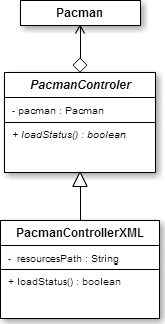
\includegraphics[width=0.3\textwidth]{images/pacmanControllerDiagram.png}
% 	\caption{Diagrama de clases con enfoque sobre \\ el controlador del pacman.}
% 	\medskip
% \end{figure}
% \bigskip

% Como se puede notar, hemos inventado un tipo de entidad denominado \textit{PacmanController}, modelizado como una clase abstracta que mantiene conocmiento de la existencia de un pacman para controlar. Esta clase es la que nos permite justamente abstraernos de la fuente de los movimientos, dándonos la posibilidad de leer estos desde un archivo (como es en nuestro caso al tomar las acciones de un archivo XML), tomar datos provenientes de una conexión de red a través de un socket, leer eventos desde el teclado, etc.
% \par
% Mas específicamente, se debe definir en el controlador que se implemente un método declarado como \textit{loadStatus()}, en donde se define desde donde provienen los movimientos, y cómo son comunicados estos al pacman. Cada vez que se invoque a dicho método, se realizará una nueva lectura de la fuente proveedora de las acciones.
% \bigskip


% % CAPITULO 3
% % Estado del juego
% \section{Estado del juego}

% Además de poder sensar los movimientos del pacman, debemos tener un mecanismo que nos permita tomar conocimiento del estado del laberinto y todo lo que en el vive, a fin de poder manipular dicha información. Estos datos pueden ser requeridos para, por ejemplo, implementar la visualización gráfica y animada del juego, o la transmisión via red de los datos para múltiples y variados propósitos.
% \par
% De esta manera, y utilizando una lógica meramente parecida a la planteada en el apartado anterior, hemos inventado un tipo de entidad \textit{LabyrinthView} modelizada como una clase abstracta. Esta tiene conocmiento del laberinto en el cual se está desarrollando el juego. Además declara un método \textit{refreshStatus()} el cual debe ser implementado por aquellas clases que se encargarán específicamente de leer la información para su utilización. El diagrama de clases de la estructura explicada se muestra en la \textit{Imagen 3.2}.
% \par
% En nuestro caso, sencillamente vamos a solicitarle al laberinto la información del estado del juego en cada tick acontecido para luego almacenarlo en un par de archivos con formato XML. Por un lado se persistirán los datos del laberinto en dicho momento, lo cual consta del almacenamiento de las distintas celdas que lo conforman, los objetos que existen en cada una de estas, etc. 
% \bigskip


% % Imagen 
% \begin{figure}[H]
% 	\centering
% 	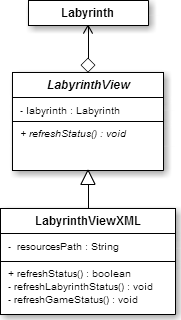
\includegraphics[width=0.3\textwidth]{images/labyrinthViewDiagram.png}
% 	\caption{Diagrama de clases con enfoque sobre \\ la vista del laberinto.}
% 	\medskip
% \end{figure}
% \bigskip


% Para evitar sobreescribir un mismo archivo, lo que significaría perder los datos de los ticks previos al último, se ha generado una secuencia de archivos XML los cuales son creados con el nombre \textit{LaberintoTick} seguido de un número que comienza a partir del 1 y que indica la correlatividad entre archivos.
% Además de la secuencia de estados del laberinto, se ha creado una secuencia de archivos XML en el que se indica el estado general del juego. Es decir, se persiste la posición del pacman en ese tick, el puntaje obtenido hasta el momento y el sentido de movimiento. Sumado a esto, se almacena el estado de cada fantasma, lo que implica el estado (e.g.: cazador), posición (fila y columna), identificador, personalidad y sentido de movimiento actual.



% %
% % CAPITULO 4
% %
% \chapter{Pruebas}


% % CAPITULO 4
% % Celdas y notificaciones
% \section{Celdas y notificaciones}

% Luego de haber diseñado el modelo para las celdas y elegido el modo que se notifican los cambios, se optó por realidad TDD sobre estos aspectos ya que involucraban varias reglas de negocio. Estas reglas fueron surgiendo a lo largo del diseño, por lo que se decidió plasmarlas en  un primer set basico de pruebas sin tener en cuenta grandes razgos y deciciones de implementación permitiendonos contemplar los limites que este alcanzaria.
% \par
% Para llevar a cabo la construcción de estas pruebas se vio necesario crear implementaciones concretas de algunas entidades abstractas para poder utilizar el comportamiento heredado e implementado en la jerarquia abstracta, como son el caso de Cell, CellObject y EatableObserver.
% \par
% En el transcurso de su implementación surgieron nuevos casos que habían sido pasados por alto debido a la profundidad de analisis que estos implicaban por lo cual se fueron agregando nuevos pero siempre respetando y validando los anteriores. Un claro ejemplo de estos casos que surgieron fue el caso de el set de celdas contiguas mostrado en el \refcode{CellTest}.


% % Código
% \lstset{ language = Java } % Cambiamos el lenguaje para que parsee en Java
% \lstinputlisting[label=CellTest,caption=``Prueba de celdas'']{codes/CellTest.java} 
% \bigskip\bigskip


% Como podemos observar, se encontró que en la configuración de celdas contiguas debe involucrar que los datos de ambas celdas no pierdan consistencia.
% \bigskip\bigskip


% % CAPITULO 4
% % Comportamiento de los fantasmas
% \section{Comportamiento de los fantasmas}

% Para probar el comportamiento de los fantasmas es necesario crear un set de celdas y una presa. Con un fantasma en estado cazador y teniendo a la presa dentro de su rango de visión, se debe probar que cada vez que se mueva lo haga de a una celda, que esta sea contigua a aquella en la que estaba previamente y que sea una celda valida, no una pared, y que la distancia con la presa haya disminuido. Lo mismo es válido para el fantasma en estado presa, solo que la distancia debe aumentar en lugar de disminuir. Si la presa no está dentro del rango de visión del fantasma, se debe probar lo mismo, con excepción de la distancia a la presa.
% \par
% En el caso del fantasma buscador, es necesario probar también que cuando la presa salga de la vista el fantasma se dirija a la celda en que lo vio por última vez. Por otro lado, en el buscador temperamental se debe probar si la visión se actualiza al cambiar la agresividad y si al volver del estado muerto al estado cazador, momento en que la agresividad toma su valor original, sucede lo mismo con la visión.
% \bigskip


% % CAPITULO 4
% % Generación de notificaciones del juego
% \section{Generación de notificaciones del juego}

% Para poder corroborar el buen funcionamiento de las notificaciones, primeramente se debió proveer al juego de un laberinto bien definido. Particularmente, se ha armado un laberinto con diez celdas de alto por diez celdas de ancho, como se muestra en la \textit{Imagen 4.1}.
% \bigskip

% % Imagen 
% \begin{figure}[H]
% 	\centering
% 	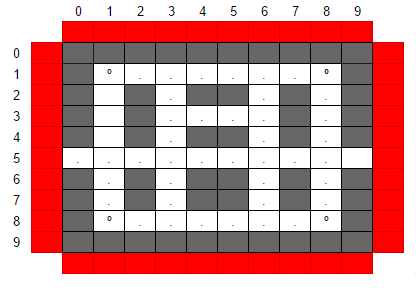
\includegraphics[width=0.6\textwidth]{images/laberintoDibujo.jpg}
% 	\caption{Diagrama visual de celdas del laberinto.}
% 	\medskip
% \end{figure}
% \bigskip


% Este laberinto se carga desde el archivo con formato XML \textit{LabyrinthConfig.xml}, y cuyo contenido puede verse en el \refcode{LaberintoXmlTest}.


% % Código
% \lstset{ language = XML } % Cambiamos el lenguaje para que parsee en XML
% \lstinputlisting[label=LaberintoXmlTest,caption=``Prueba de la serialización'']{codes/labyrinthConfig.xml} 
% \bigskip


% Para poder constatar la correcta generación de las notificaciones (serializadas en archivos XML) de los estados del laberinto y de los personajes a lo largo de los distintos ticks, se ha decidido agregar una pequeña porción de código en la aplicación misma que invoque al controlador del pacman (\refcode{SerializationTest}). Este controlador es el que hemos creado para la presente iteración, el cual lee los movimientos del pacman desde un archivo XML. De esta manera, el juego ejecutará tantos ticks como movimientos distintos se especifiquen en esta fuente de movimientos. Esta implementación se puede ver en entre las líneas 32 y 39.
% \bigskip


% % Código
% \lstset{ language = Java } % Cambiamos el lenguaje para que parsee en Java
% \lstinputlisting[label=SerializationTest,caption=``Prueba de la serialización'']{codes/SerializationTest.java} 
% \bigskip\bigskip

\end{document}
